\documentclass[11pt]{amsart}
\usepackage{amssymb, amsthm}
\usepackage{amsmath}
\usepackage[dvipsnames]{xcolor}
\usepackage{tikz}
\usetikzlibrary{arrows}
\usetikzlibrary{decorations.markings}
\tikzset{invmidarrow/.style={postaction=decorate,decoration={markings,mark={between positions 0 and 1 step #1
with {\arrow{latex reversed}}}}}}
\usetikzlibrary{shapes.geometric}

\begin{document}

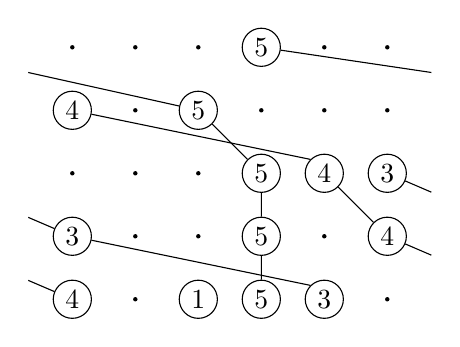
\begin{tikzpicture}[scale=0.8]
\pgfdeclarelayer{background}
\pgfdeclarelayer{foreground}
\pgfsetlayers{background,main,foreground} 

\begin{pgfonlayer}{background}
    \newcommand\rows{5}
    \newcommand\cols{6}

    % Drawing the grid with small dots
    \foreach \row in {1,...,\rows} {
        \foreach \col in {1,...,\cols} {
            \fill (\col,\row) circle (1pt); % Small filled circle
        }
    }
\end{pgfonlayer}


% Placing named balls with numbers on the foreground
\node[draw,circle,fill=white, inner sep=2pt] at (4,5) (ball5-5) {5};
\node[draw,circle,fill=white, inner sep=2pt] at (3,4) (ball5-4) {5};
\node[draw,circle,fill=white, inner sep=2pt] at (4,3) (ball5-3) {5};
\node[draw,circle,fill=white, inner sep=2pt] at (4,2) (ball5-2) {5};
\node[draw,circle,fill=white, inner sep=2pt] at (4,1) (ball5-1) {5};

\node[draw,circle,fill=white, inner sep=2pt] at (1,4) (ball4-4) {4};
\node[draw,circle,fill=white, inner sep=2pt] at (5,3) (ball4-3) {4};
\node[draw,circle,fill=white, inner sep=2pt] at (6,2) (ball4-2) {4};
\node[draw,circle,fill=white, inner sep=2pt] at (1,1) (ball4-1) {4};

\node[draw,circle,fill=white, inner sep=2pt] at (6,3) (ball3-3) {3};
\node[draw,circle,fill=white, inner sep=2pt] at (1,2) (ball3-2) {3};
\node[draw,circle,fill=white, inner sep=2pt] at (5,1) (ball3-1) {3};

\node[draw,circle,fill=white, inner sep=2pt] at (3,1) (ball1-1) {1};

% Drawing lines between named balls (wrapping around ring as needed)
\draw (ball5-5) -- (6.7, 4.6);
\draw (0.3,4.6) -- (ball5-4);
\draw (ball5-4) -- (ball5-3);
\draw (ball5-3) -- (ball5-2);
\draw (ball5-2) -- (ball5-1);

\draw (ball4-4) -- (ball4-3.135);
\draw (ball4-3) -- (ball4-2);
\draw (ball4-2) -- (6.7, 1.7);
\draw (0.3, 1.3) --(ball4-1);

\draw (ball3-3) -- (6.7, 2.7);
\draw (0.3, 2.3) -- (ball3-2);
\draw (ball3-2) -- (ball3-1.135);

\end{tikzpicture}

\end{document}